\begin{figure}
\begin{leftfullpage}
\caption[Estimation of noise correlations from population calcium signals]
{{\bf Estimation of noise correlations from population calcium signals.}
Visual stimuli comprising full-field drifting gratings interleaved with blank screens ({\bf A}) presented during two-photon recordings of somatic calcium signals using fast 3D random-access microscopy ({\bf B}).
{\bf C--F.} Calcium activity data from an example site.
{\bf C.} Representative calcium signals of seven cells, downsampled to 20 Hz, out of the 292 total recorded cells. Spiking activity inferred by nonnegative deconvolution is shown by red ticks below the trace.
{\bf D.} The spatial arrangement and orientation tuning of the 292 cells from the imaged site. The cells' colors indicate their orientation preferences. The gray cells were not significantly tuned.
{\bf E.} The sample noise correlation matrix of the activity of the neural population.
{\bf F.} Histogram of noise correlation coefficients in one site. The red line indicates the mean correlation coefficient of 0.020.
} \label{fig:2}
\end{leftfullpage}
\end{figure}

\begin{figure}
\begin{fullpage}
        \begin{center}
        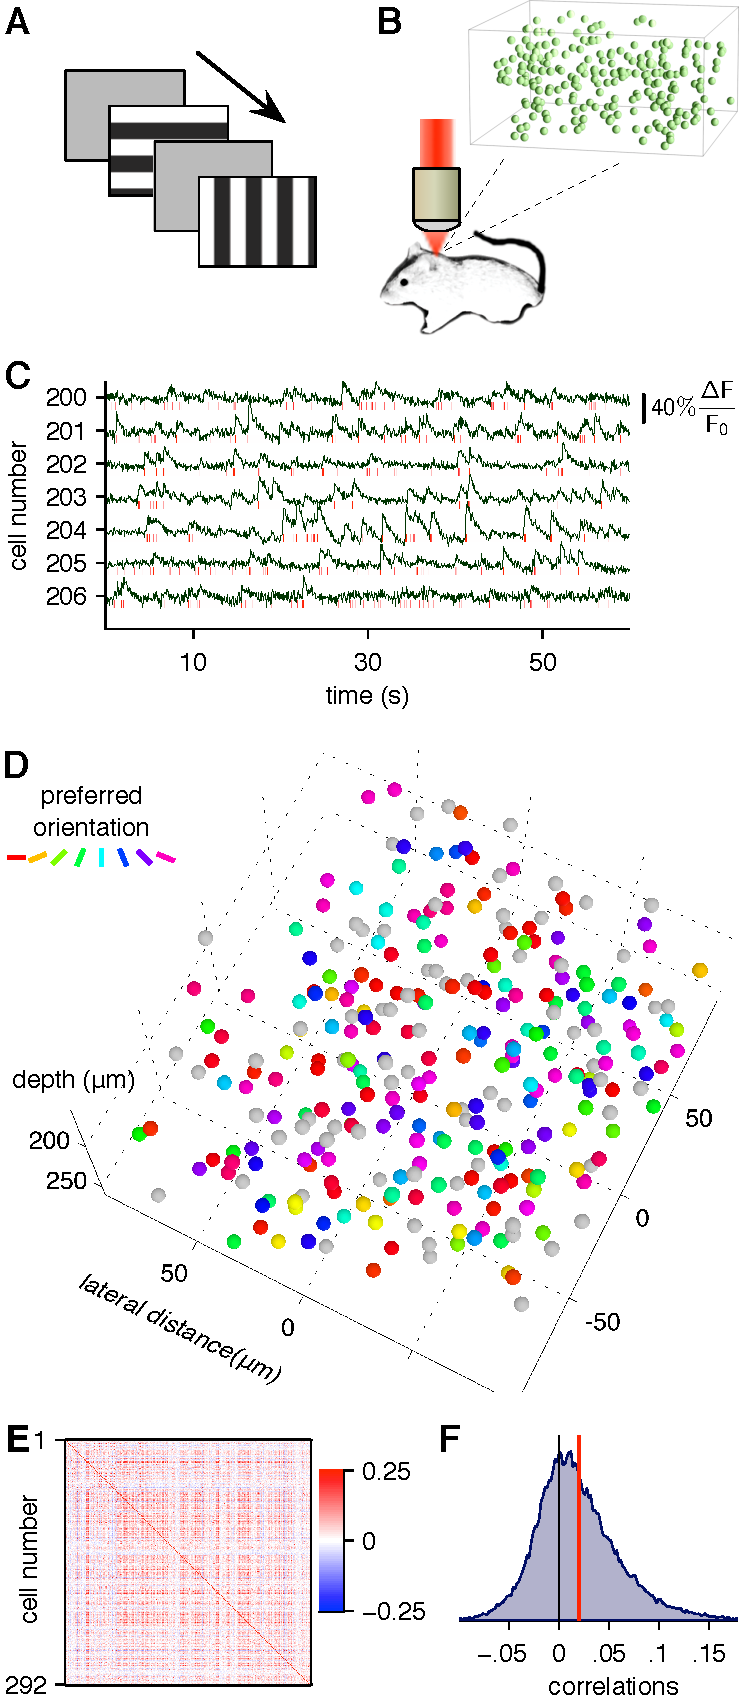
\includegraphics[height=\textheight]{./figures/Acquisition.pdf}
        \end{center}
\end{fullpage}
\end{figure}
